% !TeX spellcheck = en_US
% !TeX root = ../Tom_Sandmann-master_thesis

\appendix
\numberwithin{figure}{section}

\chapter{Appendix} \label{Appendix}

\section{Curve4Q source code additions} \label{appendix: curve4q modifications}
%
\begin{minted}[xleftmargin=\parindent, tabsize=4, obeytabs, breaklines, fontsize=\footnotesize]{python3}
# (X+Y, Y-X, Z+Z, 2d*Ta*Tb) = (X+Y, Y-X, Z+Z, 2d*Ta*Tb, -2d*Ta*Tb)
def R2ToR5(P):
    (XplusY, YminX, ZplusZ, two_dT) = P
    return(
        XplusY,
        YminX,
        ZplusZ,
        two_dT,
        GFp2.neg(two_dT)
    )


# R5toR2(X+Y, Y-X, Z+Z, 2d*Ta*Tb, -2d*Ta*Tb) = (X+Y, Y-X, Z+Z, ± 2d*Ta*Tb)
def R5toR2(P, sign):
    (XplusY, YminX, ZplusZ, two_dT, min_two_dT) = P
    # -1/+1 represented as 0/1
    options = [
        (
            YminX,
            XplusY,
            ZplusZ,
            min_two_dT
        ),
        (
            XplusY,
            YminX,
            ZplusZ,
            two_dT
        ),
    ]
    return options[sign]
\end{minted}
%  

\section{Example template traces} \label{App sec: example template traces}
\Cref{fig: OTA first iteration templates example} shows example template traces used in the first iteration of the Online Template Attack (OTA).
These traces are captured using the following base point and scalar:
%
\begin{footnotesize}
	%
	\begin{align*}
	P &= (x, y) \\
		x &= 4278750285544105074676860908476659235 + 129913138569548007992917457078809919071i \\
		y &= 18212526546888401742587968450932351321 +  43058747546351419525605575024245364232i \\
		m &= \texttt{0x5150C5D41FB74053200BBFA6A8B72032B8F48118358A215D4D9C7722E582EE6D}
	\end{align*}
	%
\end{footnotesize}
%
\begin{figure}[H]
	\centering
	\subfloat[$d_{64} = 0$]{
		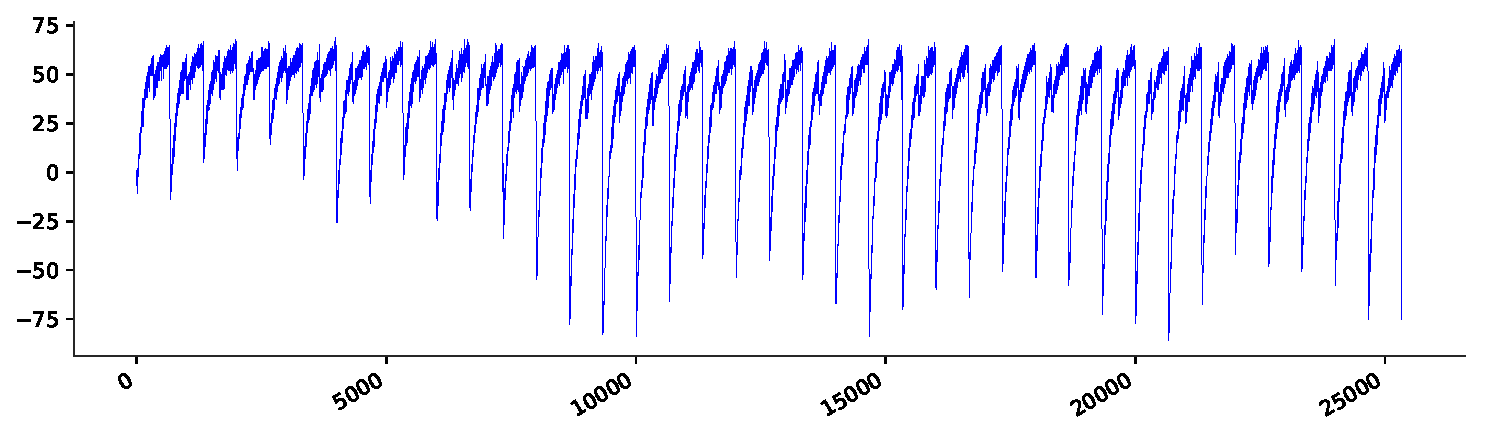
\includegraphics[scale=0.6]{traces/first_doubling/template_trace_dbl_oper_+d64_0}
	}
	\vfill
	\subfloat[$d_{64} = 1$]{
		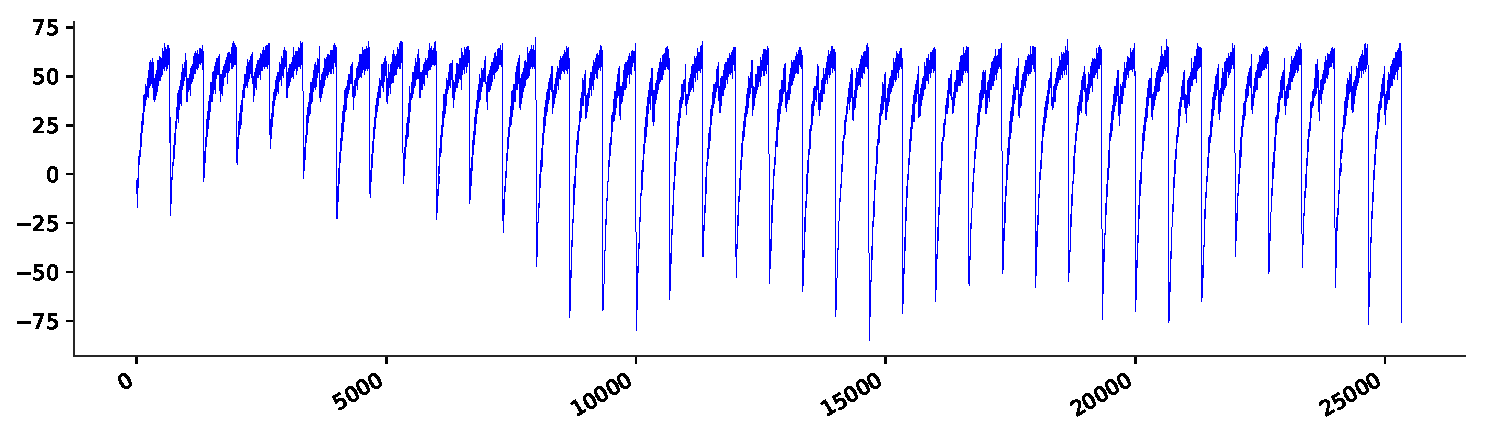
\includegraphics[scale=0.6]{traces/first_doubling/template_trace_dbl_oper_+d64_1}
	}
	\vfill
	\subfloat[$d_{64} = 2$]{
		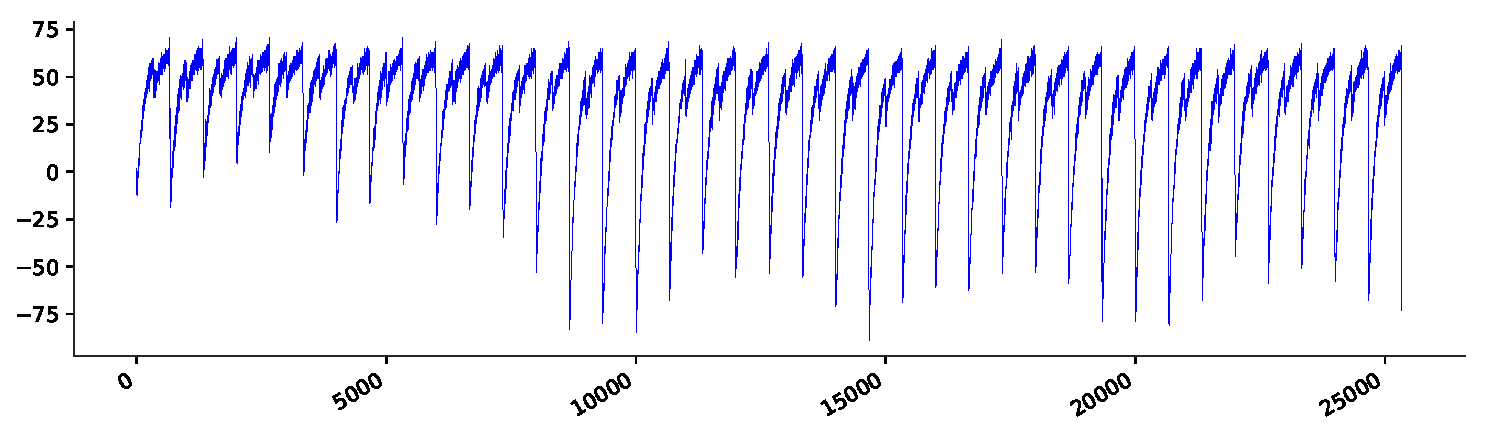
\includegraphics[scale=0.6]{traces/first_doubling/template_trace_dbl_oper_+d64_2}
	}
	\vfill
	\subfloat[$d_{64} = 3$]{
		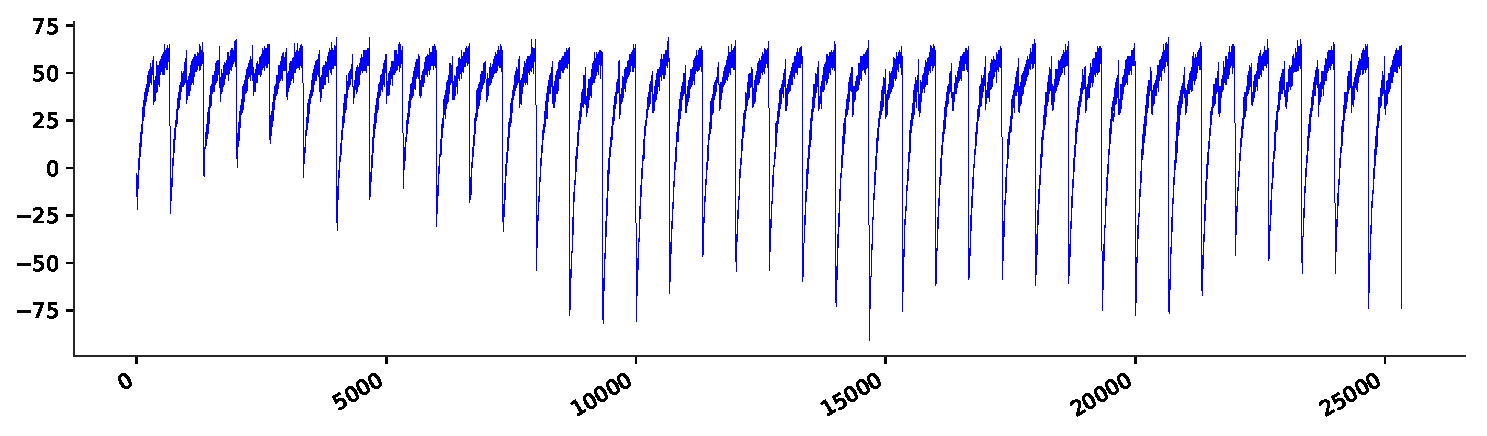
\includegraphics[scale=0.6]{traces/first_doubling/template_trace_dbl_oper_+d64_3}
	}
	\vfill
	\captionof{figure}{ }
\end{figure}
%
\begin{figure}\ContinuedFloat
	\centering
	\subfloat[$d_{64} = 4$]{
		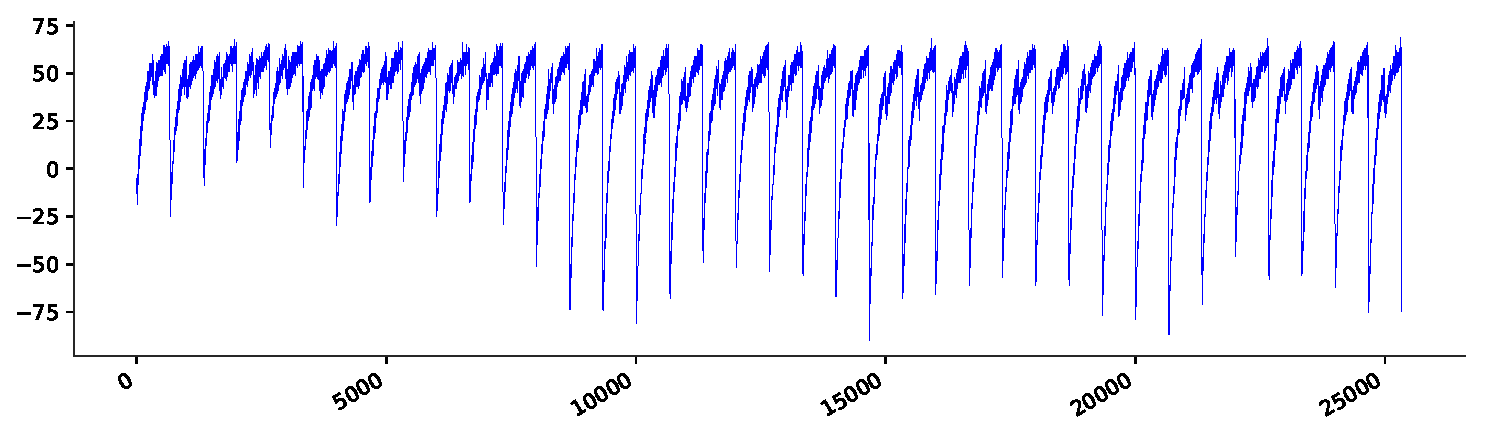
\includegraphics[scale=0.6]{traces/first_doubling/template_trace_dbl_oper_+d64_4}
	}
	\vfill
	\subfloat[$d_{64} = 5$]{
		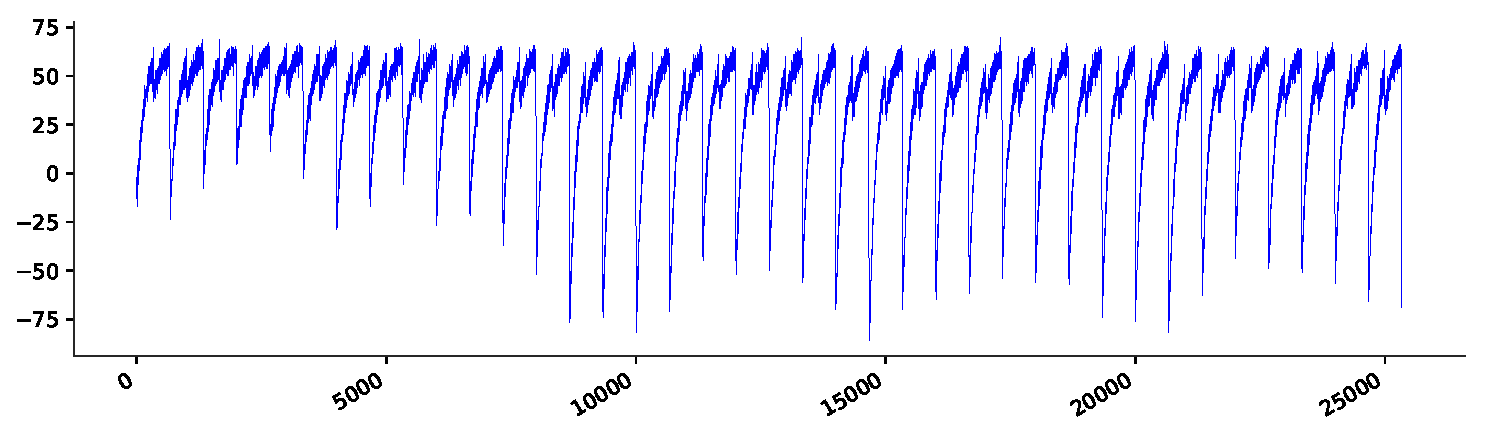
\includegraphics[scale=0.6]{traces/first_doubling/template_trace_dbl_oper_+d64_5}
	}
	\vfill
	\subfloat[$d_{64} = 6$]{
		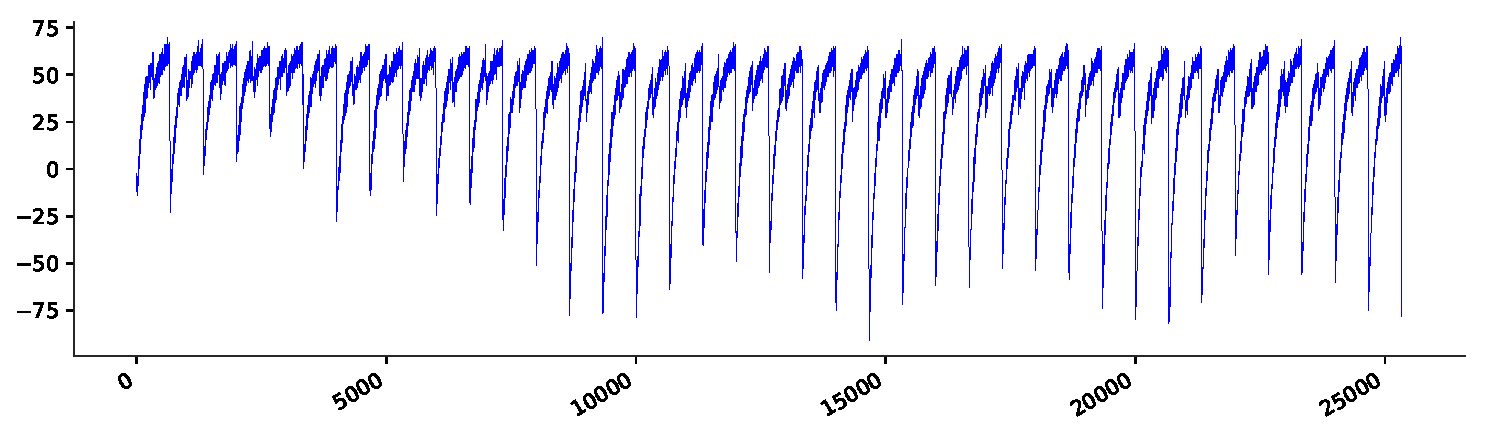
\includegraphics[scale=0.6]{traces/first_doubling/template_trace_dbl_oper_+d64_6}
	}
	\vfill
	\subfloat[$d_{64} = 7$]{
		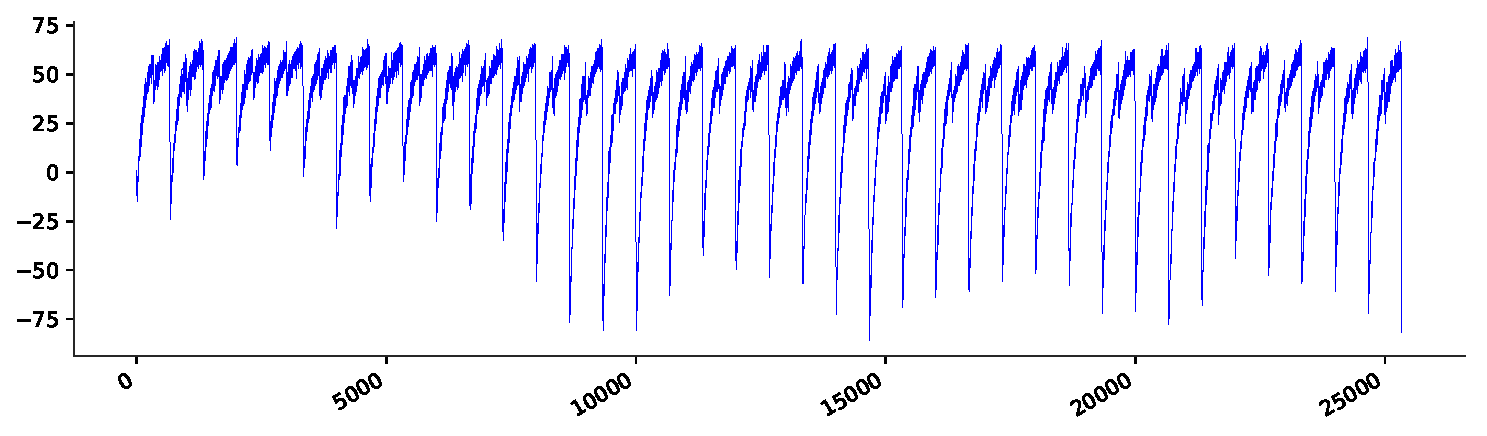
\includegraphics[scale=0.6]{traces/first_doubling/template_trace_dbl_oper_+d64_7}
	}
	\captionof{figure}{Template traces that are used to attack the first digit-column $d_{64}$ of {\fourq} using an Online Template Attack (OTA). The value of $d_{64}$ related to each template trace indicates that this was the specific value used in the doubling operation that resulted in the captured trace.}
	\label{fig: OTA first iteration templates example}
\end{figure}
%

\section{Measurement setup}
%
\begin{figure}[H]
	\centering
	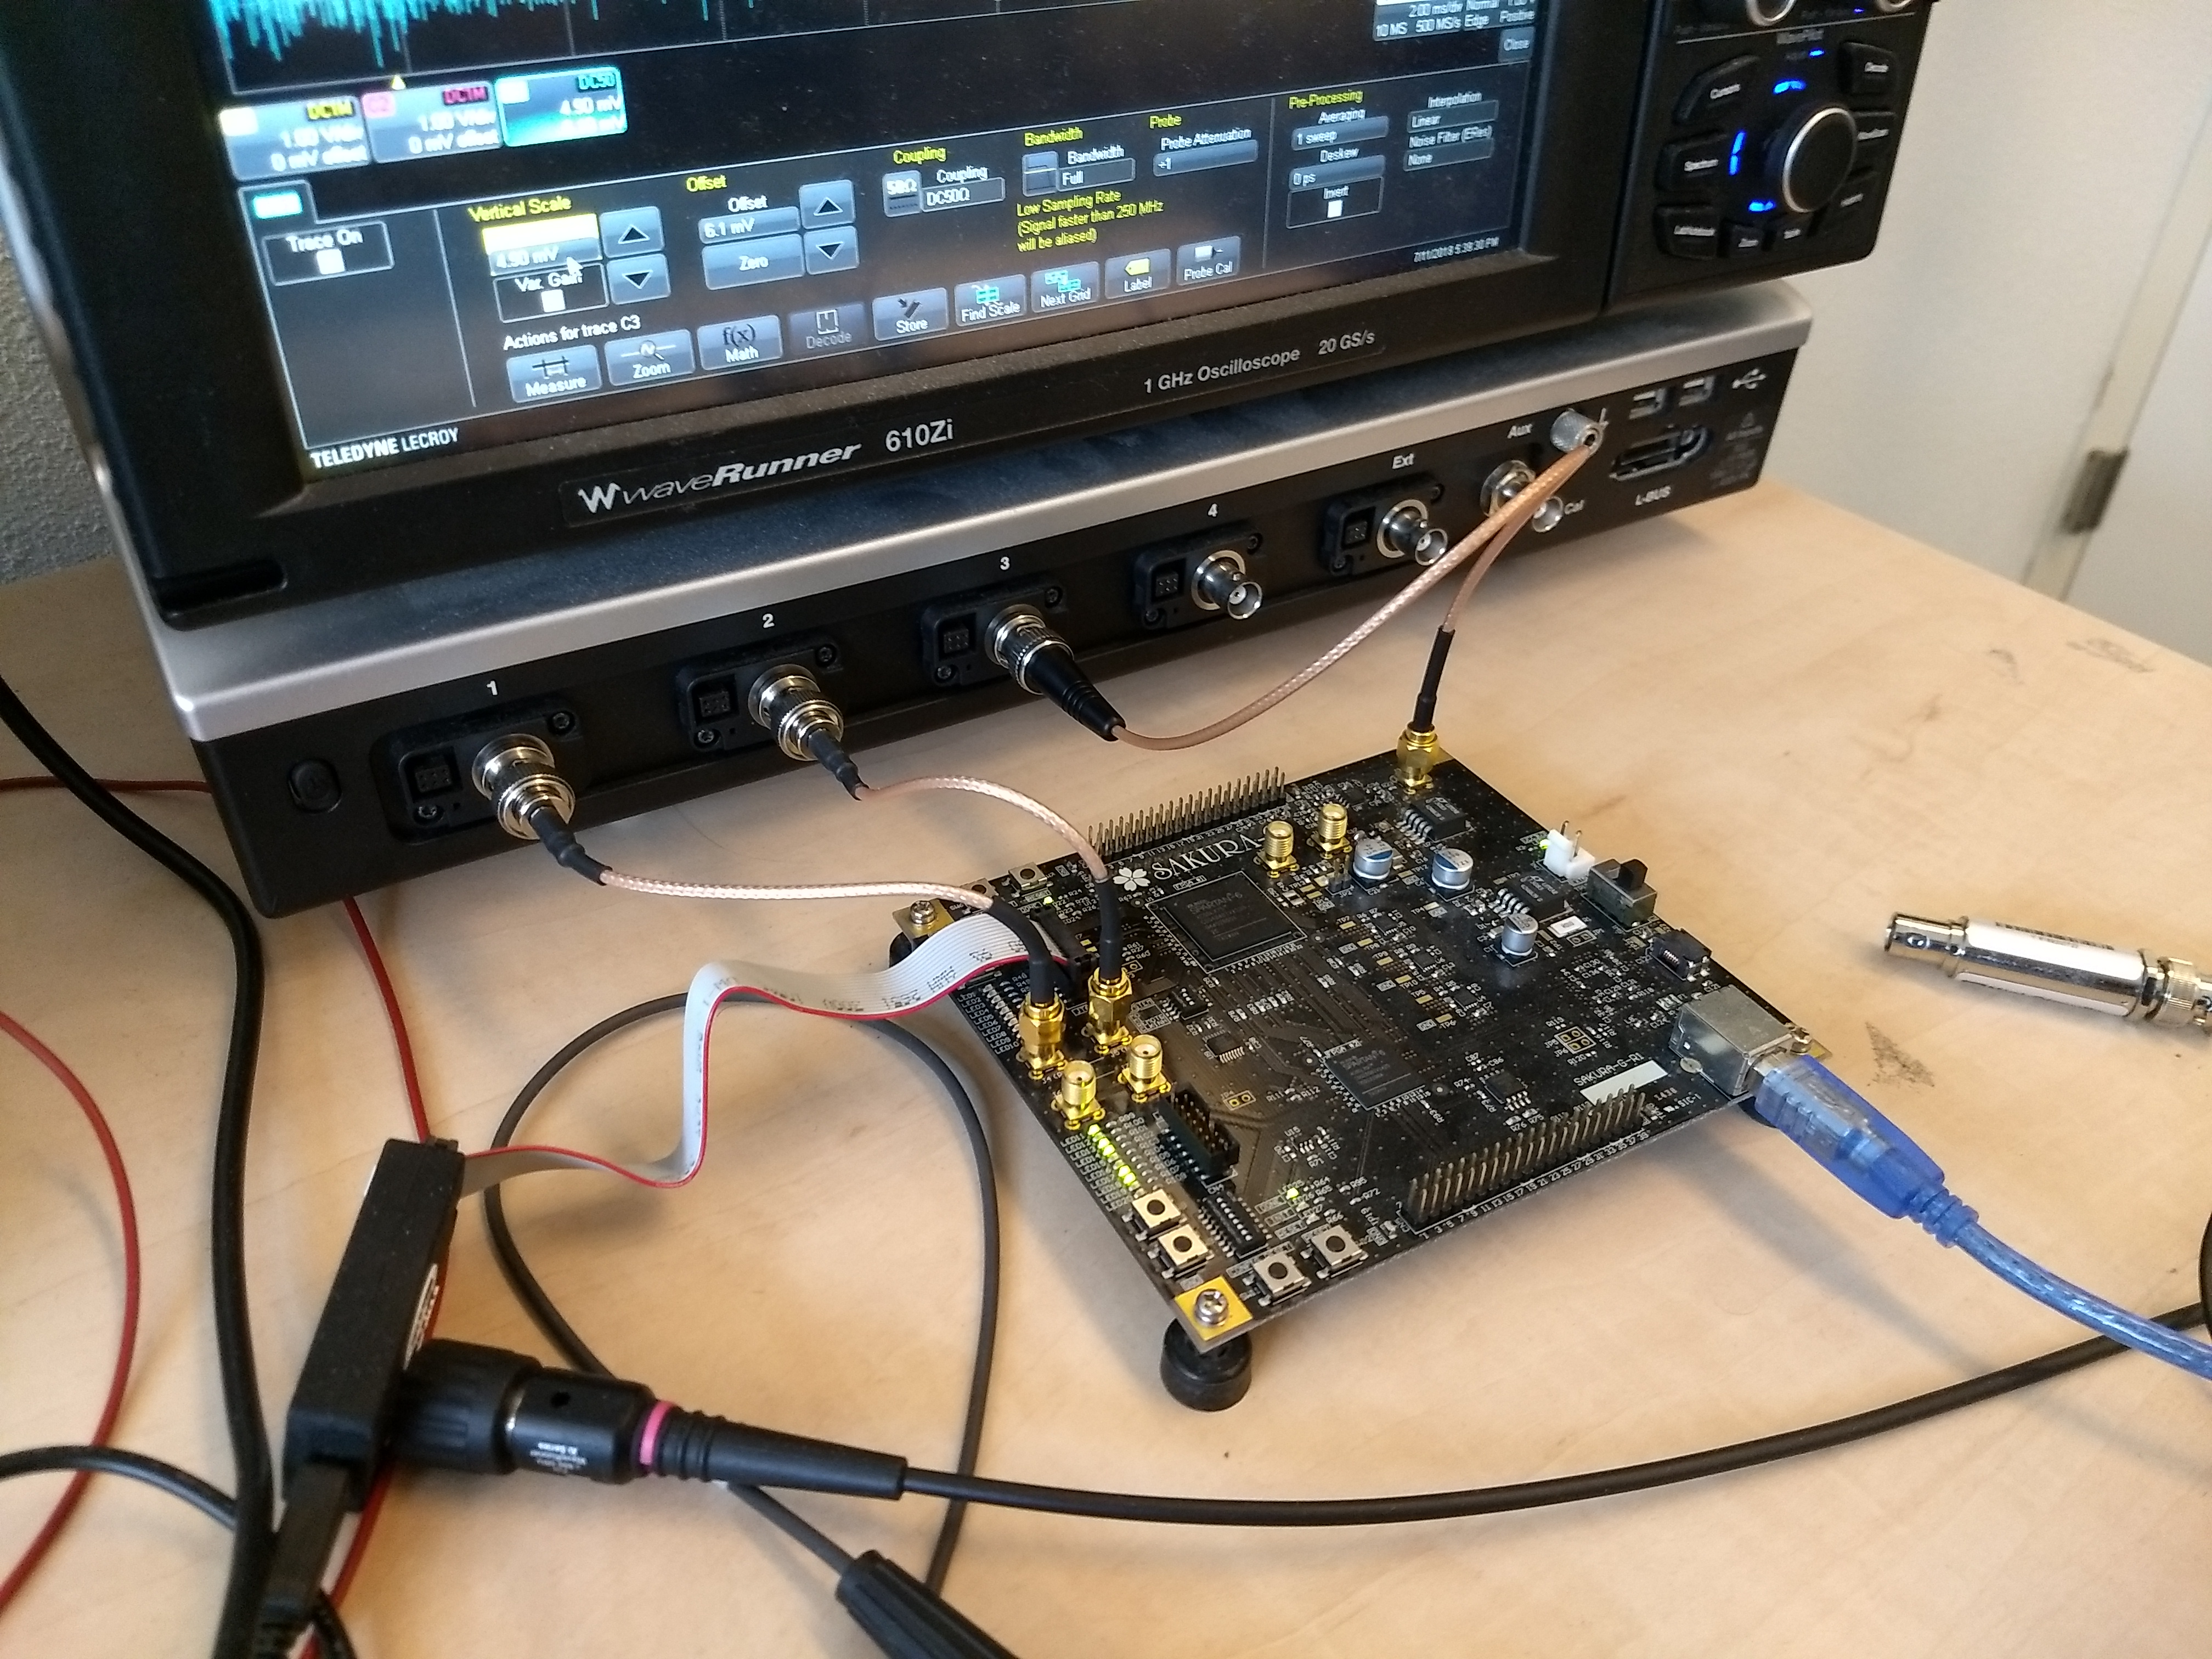
\includegraphics[scale=0.1]{setup/measurement_setup}
	\captionof{figure}{The measurement setup used to capture the power traces from the board. 
	The power output of the main FPGA is connected to $C_3$. The signal indicating the beginning and the end of the main loop is used as a trigger to capture all of the power traces. This trigger is assigned to $C_1$. Its trigger value is set to 1.00 V and it triggers on the positive edge of the signal. 
	The power trace that indicates the start and end of the doubling and addition operations in each iteration of the main loop in {\fourq} is obtained from $C_2$.
	The oscilloscope used during all of the acquisitions is the Teledyne LeCroy - WaveRunner 610Zi.
	}
\end{figure}
%

